\section{Signal and irreducible background}
\label{sec:signal}
This analysis searches for the simultaneous production of two massive bosons and a photon in a single hard scattering of a proton-proton collision at 13\TeV.
The signature of these processes varies among the three channels, but includes a number of high-momentum, isolated leptons,
with one or two pairs resonating to the Z boson mass,
and an isolated photon with high momentum.

However, there is a degree of ambiguity in what can be considered triboson production when a photon is present in the final state.
For example, in the four lepton channel, the reaction
$p p \to 4 \Pl \PGg$
has three contributions:
\begin{enumerate}
\item The photon comes from an initial state fermion (Figure \ref{fig:ppTo4LG_hard})
\item The photon comes from a Triple or Quartic Gauge Coupling (e.g. Figure \ref{fig:ppTo4LG_GC})
\item The photon is emitted as Final State Radiation (FSR) by one of the leptons from the decay of a \PZ (e.g. Figure \ref{fig:ppTo4LG_FSR})
\end{enumerate}

This analysis considers only the first and the second processes as the signal.
The third process, even though it has exactly the same particles in the final state, is part of the irreducible backgrounds.

Note that in the SM only $\PW\PZ\PGg$ can be produced via TGA/QGC

However, results will be reported both including and excluding the third contribution, by means of an additional dedicated cut described in Section \ref{sec:FSR_cut}.

\begin{figure}
  \subfigure [From initial-state fermion] {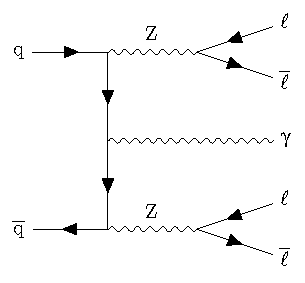
\includegraphics[width=.333333333\textwidth]{triboson_4LG.pdf} \label{fig:ppTo4LG_hard}}%
  \subfigure [From a QGC]                 {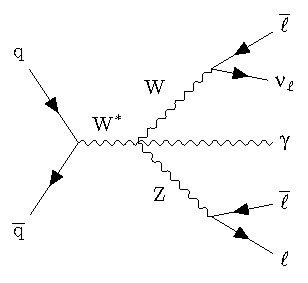
\includegraphics[width=.333333333\textwidth]{QGC_3LNuG.pdf}    \label{fig:ppTo4LG_GC}  }%
  \subfigure [From final-state fermion]   {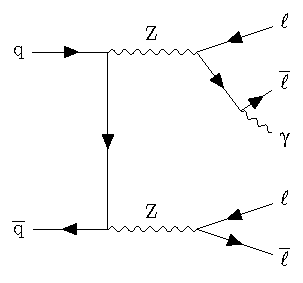
\includegraphics[width=.333333333\textwidth]{ZZ_4LG.pdf}       \label{fig:ppTo4LG_FSR} }%
\caption{Standard Model processes that yield four isolated leptons and a photon in the final state.}
\label{fig:ppTo4LG}
\end{figure}

Similarly, in the three lepton channel, only photons from the hard scattering or the ISR are part of the signal definition,
while contributions from FSR photons from one of the three leptons are part of the irreducible backgrounds.

\subsection{Signal defintion and simulation}
\note{This draft is to be checked}
The cut on the minimum \DR{} distance between the photon and the signal leptons (see Section \ref{sec:evt_photon_selection})
aims to exclude the FSR contribution.
However, a small fraction of events where the photon is emitted at large angle remains. \note{Are we sure?}
